\pdfoutput=1
\documentclass[aps,prd, amsmath,amssymb,superscriptaddress,showkeys,nofootinbib,reprint,preprintnumbers]{revtex4-1}
\usepackage{color}
\usepackage{aas_macros}
\usepackage{hyperref,breakurl}
\usepackage[usenames,dvipsnames]{xcolor}
\usepackage{dcolumn}
\usepackage{bm}
\usepackage{hyperref}
\usepackage{array}
\usepackage{dcolumn}

\usepackage{amsmath,amssymb,latexsym,times}
\DeclareMathOperator\arctanh{arctanh}

\usepackage{todonotes}
\newcommand{\verify}[1]{\textcolor{red}{\textbf{{#1}}}}

\newcommand\assign[1]{\todo[color=RoyalPurple!40, inline, size=\small]{Contributing: #1}}
\newcommand\troxel[1]{\todo[color=cyan!40, inline, size=\small]{Troxel: #1}}
 
\newcommand\green[1]{\textcolor{green}{#1}}

\begin{document}

\title{A synthetic WFIRST survey: Simulation suite and the impact of wavefront errors on weak lensing}

%\author{Troxel, M.A.}
%\email{michael.troxel@duke.edu}
\author{and others}

\collaboration{WFIRST HLS Cosmology SIT}

\noaffiliation

\date{\today}

\label{firstpage}

\begin{abstract}
\end{abstract}

\keywords{}

\maketitle

%\tableofcontents

\section{Introduction}\label{sec:intro}

DE/cosmology context

motivation for WFIRST in context of other stage iii and stage iv surveys

cosmology sit

goals of paper

\section{WFIRST and requirements}\label{sec:wfirst}

What WFIRST is \& timeline

Previous requirements information

context in broader sit work

transition to empirical validation (next section)

\def\arraystretch{1.4}
\setlength{\tabcolsep}{4pt}
\begin{table}
\caption{Table}
\label{table:values}
\begin{center}
\begin{tabular}{lcccc }
\hline
\hline
%Parameter & $o$CDM & $w$CDM & $w$CDM (Ext) & Flat Prior \\ 
%\hline
%$\Omega_m$                                                  & $0.299^{+0.024}_{-0.020}$  &  $0.300^{+0.023}_{-0.021}$  & $0.303^{+0.007}_{-0.009}$ & [0.1, 0.9] \\
%$\Omega_b$                                                   & $0.069^{+0.009}_{-0.012}$   & $0.064^{+0.013}_{-0.009}$  & $0.048^{+0.001}_{-0.001}$ & [0.03, 0.12] \\
%$\Omega_k$                                                   & $0.252^{+0.095}_{-0.14}$     & 0 & 0 & [-0.1, 0.5] \\
%$\Omega_\Lambda$                                       & $0.47^{+0.14}_{-0.12}$        & $0.700^{+0.021}_{-0.023}$  & $0.697^{+0.009}_{-0.007}$ & Derived \\
%$w$                                                                 & $-1$                                      & $-0.80^{+0.09}_{-0.11}$       & $-1.02^{+0.03}_{-0.04}$ & [-2, -0.33] \\
%$S_8$  							    & $0.801^{+0.028}_{-0.026}$  & $0.786^{+0.029}_{-0.019}$   & $0.814^{+0.016}_{-0.011}$ & Derived \\ 
\hline
\hline
\end{tabular}
\end{center}
\end{table}

\begin{figure*}
\begin{center}
\includegraphics[width=\textwidth]{figures/fov.pdf}
\end{center}
\caption[]{
Simulated field-of-view. (give info about size) (obviously chip orientation is still wrong in this...
\label{fig:fov}}
\end{figure*}


\begin{figure}
\begin{center}
\includegraphics[width=\columnwidth]{figures/sca1.png}
\end{center}
\caption[]{
sca 10
\label{fig:sca}}
\end{figure}

\begin{figure}
\begin{center}
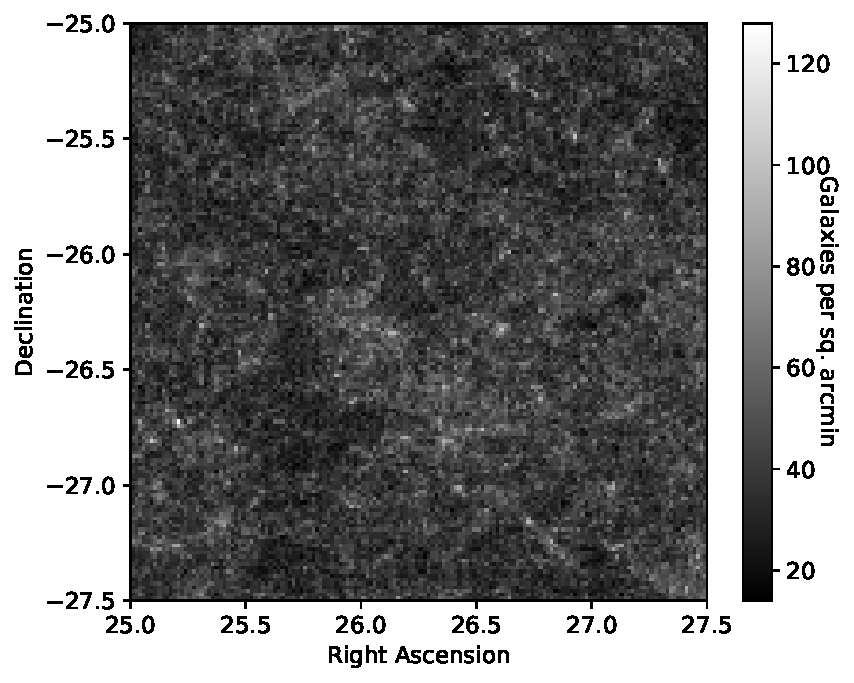
\includegraphics[width=\columnwidth]{figures/galaxies.pdf}
\end{center}
\caption[]{
Galaxies, avg. 40 per sq arcmin, dist. from buzzard, phot/morph props from candels catalog
\label{fig:galaxies}}
\end{figure}

\begin{figure}
\begin{center}
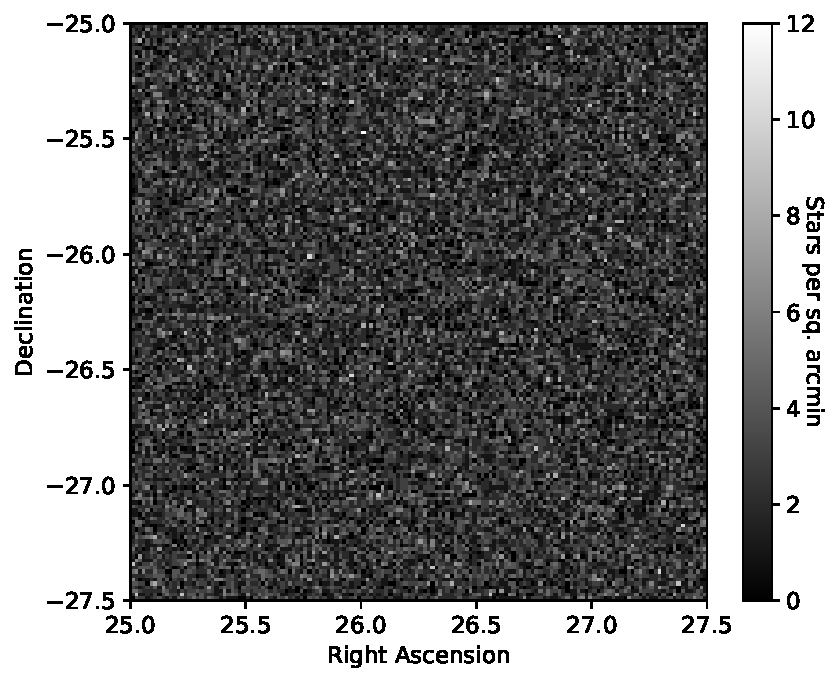
\includegraphics[width=\columnwidth]{figures/stars.pdf}
\end{center}
\caption[]{
Stars, avg. 2.5 per sq. arcmin, from galaxia
\label{fig:stars}}
\end{figure}

\begin{figure*}
\begin{center}
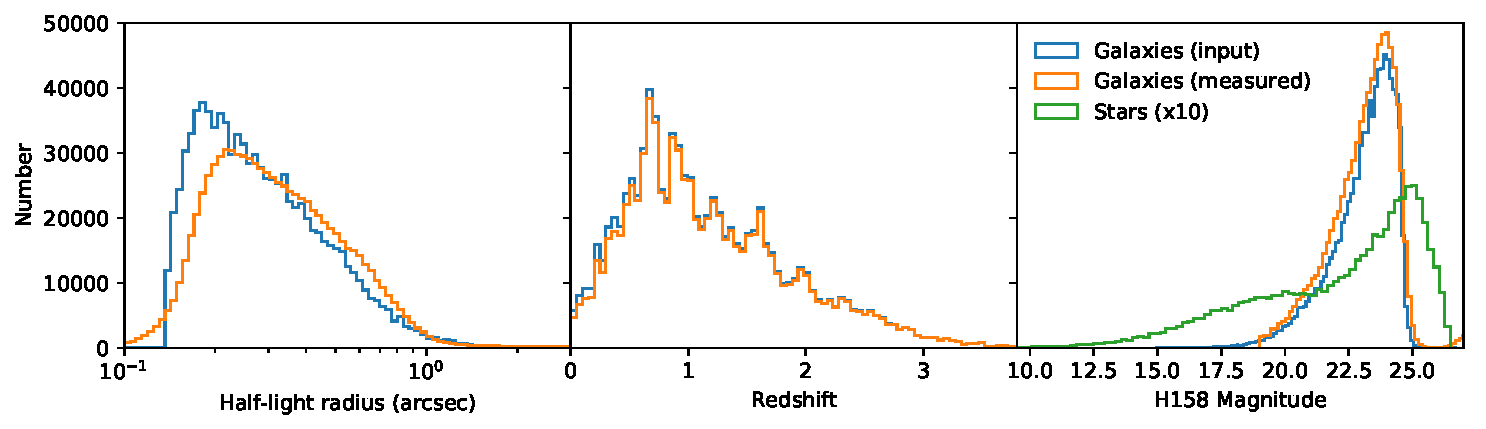
\includegraphics[width=\textwidth]{figures/hist.pdf}
\end{center}
\caption[]{
True galaxy and star properties.
\label{fig:hist}}
\end{figure*}

\begin{figure}
\begin{center}
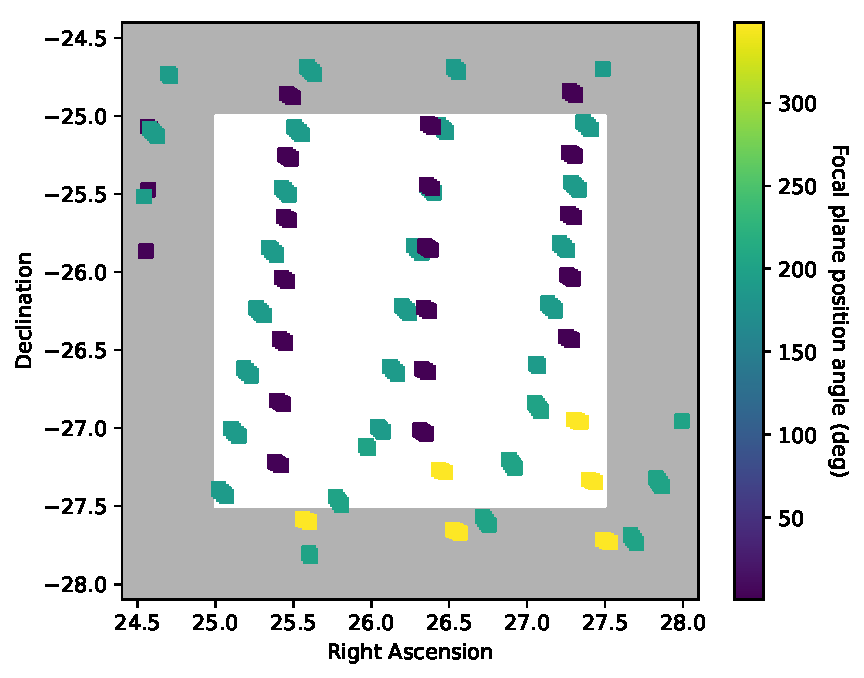
\includegraphics[width=\columnwidth]{figures/pointings.pdf}
\end{center}
\caption[]{
Pointings that overlap the simulated region (non-shaded). The color of each marker shows the position angle of the focal plane.
\label{fig:pointings}}
\end{figure}

\begin{figure*}
\begin{center}
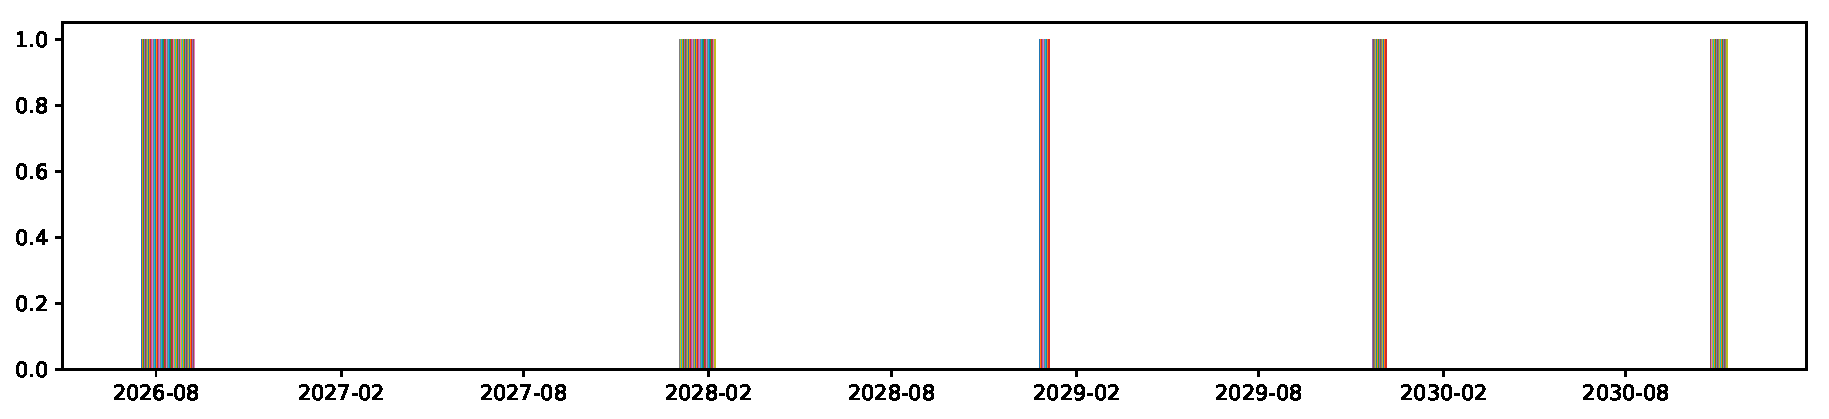
\includegraphics[width=\textwidth]{figures/dates.pdf}
\end{center}
\caption[]{
Dates of observations (is this useful? hard to make it readable)
\label{fig:dates}}
\end{figure*}

\begin{figure}
\begin{center}
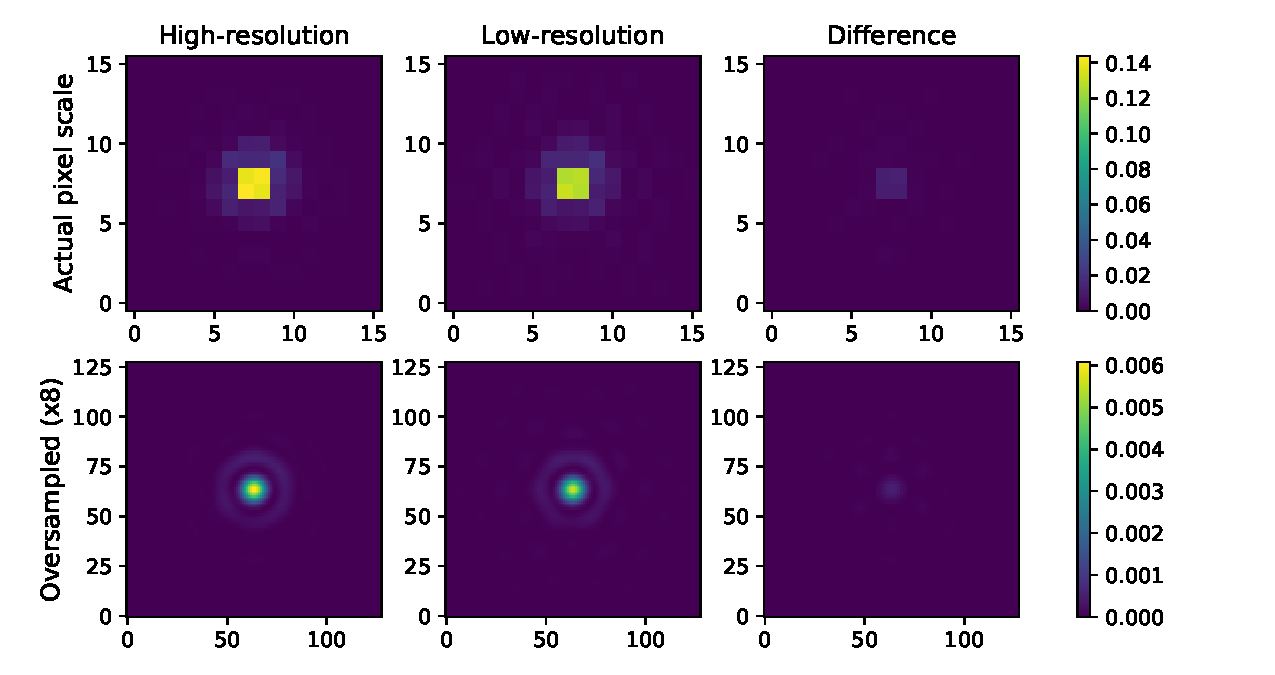
\includegraphics[width=\columnwidth]{figures/psf.pdf}
\end{center}
\caption[]{
Example oversampled PSF model compared to native pixel PSF, SCA 1. Top row - full resolution, bottom row - approx. used in sim, left - native pixel scale, right - oversample factor 8
\label{fig:pointings}}
\end{figure}


\section{Simulation suite}\label{sec:sim}



into to a synthetic survey and necessary components

galsim framework and cycle 7 (\verify{6?}) baseline

Detailed description of simulation suite components

\subsection{GalSim}
\subsubsection{Implemented detector effects}
\subsection{Galaxy catalog}
\subsection{Star catalog}
\subsection{Survey strategy}

\section{Impact of wavefront errors}\label{sec:results}

background on psf and wavefront errors

details of wfirst psf in cycle 7 (\verify{6?}) baseline

summary of approach 

\subsection{Static biases}\label{sec:static}

Describe static bias cases

\subsection{High-frequency biases}\label{sec:low}

Describe high-frequency bias cases

\subsection{Low-frequency biases}\label{sec:high}

Describe low-frequency bias cases

\subsection{results}\label{sec:results}

present results in some way

\section{Conclusion}\label{sec:conclusion}

wrap-up

future work and timeline

\section*{Acknowledgements}

This work used resources on the CCAPP condo of the Ruby Cluster at the Ohio Supercomputing Center \cite{OhioSupercomputerCenter1987} and ...OSG, Duke.... Plots in this manuscript were produced partly with \textsc{Matplotlib} \cite{Hunter:2007}, and it has been prepared using NASA's Astrophysics Data System Bibliographic Services.

\bibliographystyle{apsrev4-1}
\bibliography{wfirst_imsim_paper1}

\label{lastpage}

\end{document}
